\section{Interprete}
\subsection{Diagrammi della classi}
L'interprete è la componente di \glossaryItem{MaaS} che si occupa della conversione da \glossaryItem{DSL} Structure in \glossaryItem{DSL}. Questa decisione è stata presa per poter avere una rappresentazione semplice da manipolare attraverso l'editor e facile da ricondurre nel formato testuale.

La progettazione ha seguito un approccio bottom-up, a partire dalla creazione delle componenti per il funzionamento, includendole in un \glossaryItem{package} e inserendo un \textit{Facade} per semplificarne l'uso. Sono stati usati i pattern \textit{Facade}, \textit{Singleton} e \textit{Chain of Responsability}.
\subsection{Package DSLInterpreter}
\begin{figure}[H]
  \centering
  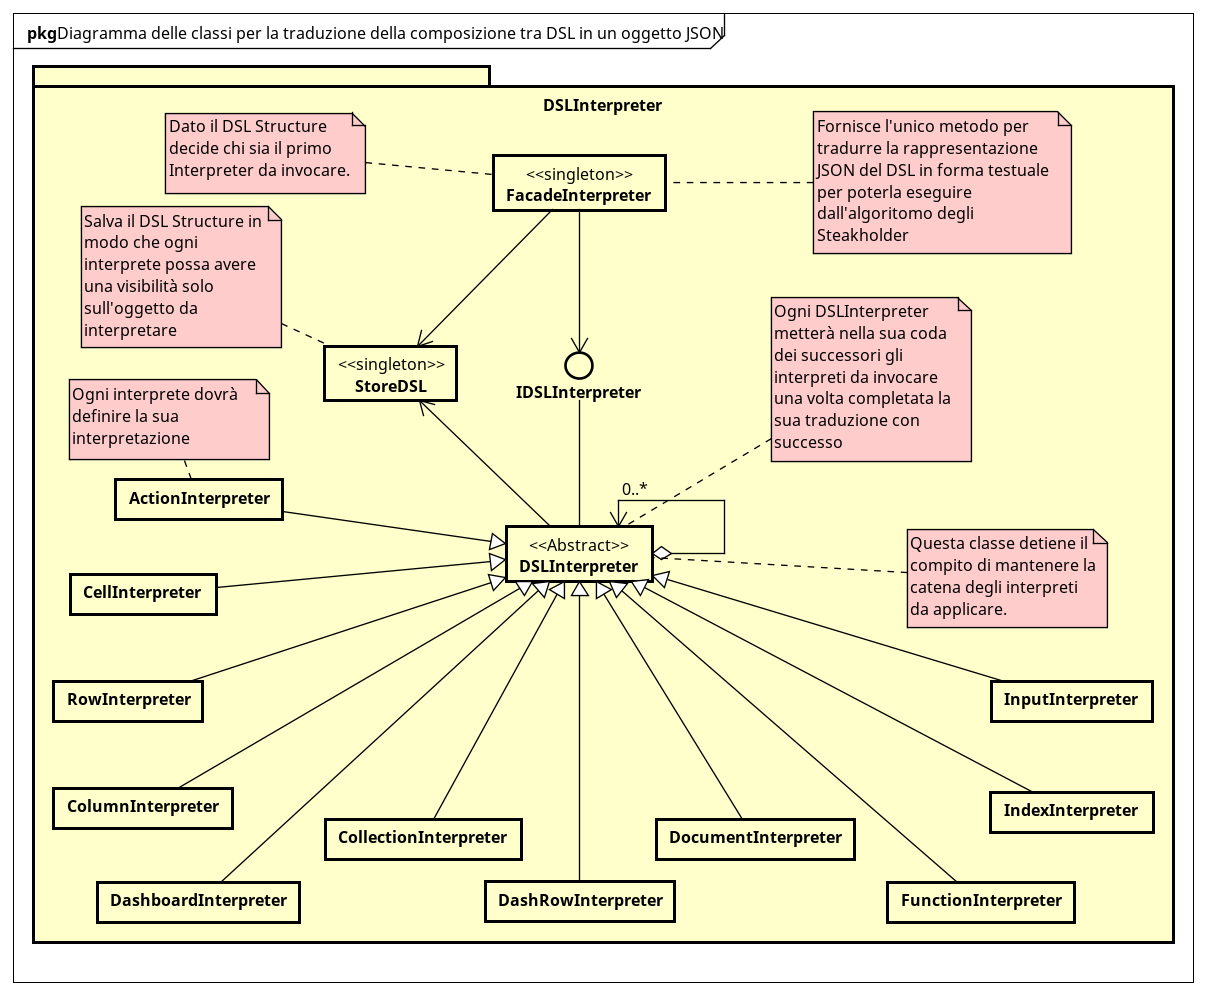
\includegraphics[width=0.9\textwidth]{res/img/Diagram_Interpreter.png}
  \caption{Package DSLInterpreter}
  \label{fig:diagram_interpreter}
\end{figure}
\subsubsection{Descrizione}
In questo \glossaryItem{package} vengono inserite tutte le classi che contribuiscono alla traduzione dal \glossaryItem{DSL} Structure prodotto dall'editor all'equivalente specifica \glossaryItem{DSL}.
La classe DSLInterpreter implementa il \textit{Chain of Responsability} e detiene una lista di tutti gli interpreti da invocare man mano che vengono applicate le traduzioni. Il risultato di ogni interprete verrà contatenato e come risultato si otterrà la specifica \glossaryItem{DSL} richiesta.
Il FacadeInterpreter implementa il pattern \textit{Facade} per offrire un'interfaccia semplice per attuare la traduzione rendendo nascoste i componenti per applicarla.
\subsubsection{DSLInterpreter::FacadeInterpreter}
\begin{itemize}
\item \textbf{Descrizione} \hfill \\
  Rappresenta l'implementazione del pattern \textit{Facade}.
\item \textbf{Utilizzo} \hfill \\
  Permette di interfacciarsi al \glossaryItem{modulo} richiedendo eslusivamente la traduzione da \glossaryItem{DSL} Structure a specifica \glossaryItem{DSL}. Questo oltre a semplificare al \textit{client} la gestione della traduzione, nasconde l'implementazione rendendo il \glossaryItem{modulo} maggiormente manutenibile.
\item \textbf{Relazioni con altre classi} \hfill
  \begin{itemize}
  \item DSLInterpreter::StoreDSL - Invocata per salvare la definizione della DSL Structure
  \item DSLInterpreter::IDSLInterpreter - Riferimento all'interpretere da eseguire. Si determina il tipo del DSL Element, ne si crea un'istanza e si invoca il metodo di traduzione
  \end{itemize}
\end{itemize}
\subsubsection{DSLInterpreter::StoreDSL}
\begin{itemize}
\item \textbf{Descrizione} \hfill \\
  Mantiene il riferimento del \glossaryItem{DSL} Structure da tradurre.
\item \textbf{Utilizzo} \hfill \\
  Viene usata dalle implementazioni di \texttt{DSLInterpreter::DSLInterpreter} per ottenere l'oggetto riferito su un attributo della struttura da tradurre. Questi \glossaryItem{casi} si riscontrano nella definizione di un componente del \glossaryItem{DSL} in cui sono innestati altri componenti ( es. \glossaryItem{Collection} con \glossaryItem{Index} e \glossaryItem{Document} ).

  Ciò permette di non violare il \textit{Single Responsability Principle}, in quanto i vari interpreti conoscono solo una singola struttura da tradurre e non detengono un possibile accesso all'intera \glossaryItem{DSL} Structure.
\item \textbf{Relazione con altre classi} \hfill
  \begin{itemize}
  \item DSLInterpreter::DSLFacadeInterpreter - Invoca il metodo per salvare la DSL Structure
  \item DSLInterpreter::DSLInterpreter - 
  \end{itemize}
\end{itemize}
\subsubsection{DSLInterpreter::DSLInterpreter}
\begin{itemize}
\item \textbf{Descrizione} \hfill \\
  Classe astratta nel quale viene richiesta l'implementazione della traduzione di un oggetto a \glossaryItem{DSL}. Da qui verranno derivati gli interpreti per ogni \glossaryItem{DSL} Element.
\item \textbf{Utilizzo} \hfill \\
  Implementa il \textit{Chain of Responsability}, mantenendo la lista degli interpreti da eseguire. In più detiene la sequenza di passi per portare a compimento la traduzione.
\item \textbf{Relazione con altre classi} \hfill
  \begin{itemize}
  \item DSLInterpreter::FacadeInterpreter
  \item DSLInterpreter::StoreDSL
  \item DSLInterpreter::ActionInterpreter
  \item DSLInterpreter::CellInterpreter
  \item DSLInterpreter::RowInterpreter
  \item DSLInterpreter::ColumnInterpreter
  \item DSLInterpreter::DashboardInterpreter
  \item DSLInterpreter::CollectionInterpreter
  \item DSLInterpreter::DashRowInterpreter
  \item DSLInterpreter::DocumentInterpreter
  \item DSLInterpreter::FunctionInterpreter
  \item DSLInterpreter::IndexInterpreter
  \item DSLInterpreter::InputInterpreter
  \end{itemize}
\end{itemize}

\subsubsection{DSLInterpreter::ActionInterpreter}
\begin{itemize}
\item \textbf{Descrizione} \hfill \\
Implementa la traduzione di un oggetto che abbia le caratteristiche di un \glossaryItem{Action} Element.
\item \textbf{Utilizzo} \hfill \\
Usato da \texttt{DSLInterpreter::CollectionInterpreter} e \texttt{DSLInterpreter::Document-}\\\texttt{Interpreter} per tradurre un attributo di tipo \glossaryItem{Action} Element associato.
\item \textbf{Relazone con altre classi}
\begin{itemize}
\item DSLInterpreter::DSLInterpreter
\item DSLInterpreter::CollectionInterpreter
\item DSLInterpreter::DocumentInterpreter
\end{itemize}
\end{itemize}

\subsubsection{DSLInterpreter::CellInterpreter}
\begin{itemize}
\item \textbf{Descrizione} \hfill \\
Implementa la traduzione di un oggetto che abbia le caratteristiche di un \glossaryItem{Cell} Element.
\item \textbf{Utilizzo} \hfill \\
Usato da \texttt{DSLInterpreter::FacadeInterpreter} nel caso un \glossaryItem{Cell} Element fosse l'elemento radice del \glossaryItem{DSL} Structure, altrimenti viene creato da \\\texttt{DSLInterpreter::DashRowInterpreter} quando un \glossaryItem{Cell} Element compone una riga della \glossaryItem{Dashboard} Element.
\item \textbf{Relazione con altre classi}
\begin{itemize}
\item DSLInterpreter::FacadeInterpreter
\item DSLInterpreter::DSLInterpreter
\item DSLInterpreter::StoreDSL
\item DSLInterpreter::DashRowInterpreter
\item DSLInterpreter::InputInterpreter
\end{itemize}
\end{itemize}

\subsubsection{DSLInterpreter::RowInterpreter}
\begin{itemize}
\item \textbf{Descrizione} \hfill \\
Implementa la traduzione di un oggetto che abbia le caratteristiche di un \glossaryItem{Row} Element.
\item \textbf{Utilizzo} \hfill \\
Usato da \texttt{DSLInterpreter::DocumentInterpreter} per tradurre un attributo \glossaryItem{Row} Element associato.
\item \textbf{Relazione con altre classi}  
\begin{itemize}
\item DSLInterpreter::DSLInterpreter
\item DSLInterpreter::DocumentInterpreter
\end{itemize}
\end{itemize}

\subsubsection{DSLInterpreter::ColumnInterpreter}
\begin{itemize}
\item \textbf{Descrizione} \hfill \\
Implementa la traduzione di un oggeto che abbia le caratteristiche di un \glossaryItem{Column} Element.
\item \textbf{Utilizzo} \hfill \\
Usato da \texttt{DSLInterpreter::IndexInterpreter} per tradurre un attributo di tipo \glossaryItem{Column} Element associato.
\item \textbf{Relazione con altre classi}
\begin{itemize}
\item DSLInterpreter::DSLInterpreter
\item DSLInterpreter::IndexInterpreter
\end{itemize}
\end{itemize}

\subsubsection{DSLInterpreter::DashboardInterpreter}
\begin{itemize}
\item \textbf{Descrizione} \hfill \\
Implementa la traduzione di un oggetto che abbia le caratteristiche di un \glossaryItem{Dashboard} Element.
\item \textbf{Utilizzo} \hfill \\
Usato da \texttt{DSLInterpreter::FacadeInterpreter} nel caso un \glossaryItem{Dashboard} Element fosse l'elemento radice del \glossaryItem{DSL} Structure. 
\item \textbf{Relazione con altre classi}
\begin{itemize}
\item DSLInterpreter::DSLInterpreter
\item DSLInterpreter::FacadeInterpreter
\item DSLInterpreter::StoreDSL
\item DSLInterpreter::DashRowInterpreter
\end{itemize}
\end{itemize}

\subsubsection{DSLInterpreter::CollectionInterpreter}
\begin{itemize}
\item \textbf{Descrizione} \hfill \\
Implemenata la traduzione di un oggetto che abbia le caratteristiche di un \glossaryItem{Collection} Element.
\item \textbf{Utilizzo} \hfill \\
  Usato da \texttt{DSLInterpreter::FacadeInterpreter} \newline nel caso un \glossaryItem{Collection} Element fosse l'elemento radice del \glossaryItem{DSL} Structure, altrimenti viene creato da \texttt{DSLInterpreter::DashRowInterpreter} \newline quando un \glossaryItem{Collection} Element compone una riga della \glossaryItem{Dashboard} Element.
\item \textbf{Relazione con altre classi}
\begin{itemize}
\item DSLInterpreter::DSLInterpreter
\item DSLInterpreter::FacadeInterpreter
\item DSLInterpreter::StoreDSL
\item DSLInterpreter::IndexInterpreter
\item DSLInterpreter::DocumentInterpreter
\item DSLInterpreter::ActionInterpreter
\end{itemize}
\end{itemize}

\subsubsection{DSLInterpreter::DashRowInterpreter}
\begin{itemize}
\item \textbf{Descrizione} \hfill \\
Implementa la traduzione di un oggeto che abbia le caratteristiche di un \glossaryItem{DashRow Element}.
\item \textbf{Utilizzo} \hfill \\
Usato da \texttt{DSLInterpreter::DashboardInterpreter} per tradurre un attributo di tipo \glossaryItem{DashRow Element} associato.
\item \textbf{Relazione con altre classi}
\begin{itemize}
\item DSLInterpreter::DSLInterpreter
\item DSLInterpreter::StoreDSL
\item DSLInterpreter::DashboardInterpreter
\item DSLInterpreter::CellInterpreter
\item DSLInterpreter::CollectionInterpreter
\item DSLInterpreter::DocumentInterpreter
\end{itemize}
\end{itemize}

\subsubsection{DSLInterpreter::DocumentInterpreter}
\begin{itemize}
\item \textbf{Descrizione} \hfill \\
  Implementa la traduzione di un oggetto che abbia le caratteristiche di un \glossaryItem{Document} Element.
\item \textbf{Utilizzo} \hfill \\
Usato da \texttt{DSLInterpreter::FacadeInterpreter} nel caso un \glossaryItem{Document} Element fosse l'elemento radice del \glossaryItem{DSL} Structure, altrimenti viene creato da \\\texttt{DSLInterpreter::DashRowInterpreter} quando un \glossaryItem{Document} Element compone una riga della \glossaryItem{Dashboard} Element.
\item \textbf{Relazione con altre classi}
  \begin{itemize}
  \item DSLInterpreter::DSLInterpreter
  \item DSLInterpreter::FacadeInterpreter
  \item DSLInterpreter::StoreDSL
  \item DSLInterpreter::CollectionInterpreter
  \item DSLInterpreter::RowInterpreter
  \item DSLInterpreter::ActionInterpreter
  \end{itemize}
\end{itemize}

\subsubsection{DSLInterpreter::FunctionInterpreter}
\begin{itemize}
\item \textbf{Descrizione} \hfill \\
  Implementa la traduzione di un oggetto che abbia le caratteristiche di un \glossaryItem{Function Element}.
\item \textbf{Utilizzo} \hfill \\
  Usato dal \texttt{DSLInterpreter::FacadeInterpreter} per tradurre i \glossaryItem{Function Element} dichiarati nella \glossaryItem{DSL} Structure.
\item \textbf{Relazione con altre classi}
  \begin{itemize}
  \item DSLInterpreter::DSLInterpreter
  \item DSLInterpreter::FacadeInterpreter
  \end{itemize}
\end{itemize}

\subsubsection{DSLInterpreter::IndexInterpreter}
\begin{itemize}
\item \textbf{Descrizione} \hfill \\
  Implementa la traduzione di un oggetto che abbia le caratteristiche di un \glossaryItem{Index} Element.
\item \textbf{Utilizzo} \hfill \\
  Usato da \texttt{DSLInterpreter::CollectionInterpreter} per tradurre un attributo di tipo \glossaryItem{Index} Element associato.
\item \textbf{Relazione con altre classi}
  \begin{itemize}
  \item DSLInterpreter::DSLInterpreter
  \item DSLInterpreter::StoreDSL
  \item DSLInterpreter::CollectionInterpreter
  \item DSLInterpreter::ColumnInterpreter
  \end{itemize}
\end{itemize}

\subsubsection{DSLInterpreter::InputInterpreter}
\begin{itemize}
\item \textbf{Descrizione} \hfill \\
  Implementa la traduzione di un oggetto che abbia le caratteristiche di un \glossaryItem{Input Element}.
\item \textbf{Utilizzo} \hfill \\
  Usato da \texttt{DSLInterpreter::IndexInterpreter}, \texttt{DSLInterpreter::CellInterpreter} e da se stesso (data la struttura ricorsiva) per tradurre un attributo di tipo \glossaryItem{Input Element} associato.
\item \textbf{Relazione con altre classi}
  \begin{itemize}
  \item DSLInterpreter::DSLInterpreter
  \item DSLInterpreter::StoreDSL
  \item DSLInterpreter::CellInterpreter
  \item DSLInterpreter::CollectionInterpreter
  \item DSLInterpreter::InputInterpreter
  \end{itemize}
\end{itemize}
